

\section[Applications]{Applications of Semantic Similarity Measures}
\subsection{Lexico-Semantic Search}


\begin{frame}
\frametitle{Related publications}
\begin{itemize}
\item Panchenko A., Romanov P., Morozova O., Naets H., Philippovich A., Fairon
C. \textbf{Serelex: Search and Visualization of Semantically Related Words}.
In Proceedings of the 35th European Conference on Information Retrieval (ECIR 2013), Moscow (Russia), 2013.

\item Panchenko A., Naets H., Brouwers L., Romanov P., Fairon C., \textbf{Recherche et visualisation de mots sémantiquement li\'{e}s}. Actes de la 20e conf\'{e}rence sur le Traitement Automatique des Langues Naturelles (TALN'2013). Les Sables d'Olonne, France. pp.747--754, 2013.

\end{itemize}
\end{frame}




\begin{frame}
\frametitle{Search for Related Words: the List and the Graph}

\begin{itemize}
\item \url{http://serelex.org}
\end{itemize}


\begin{figure}	
	\centering
	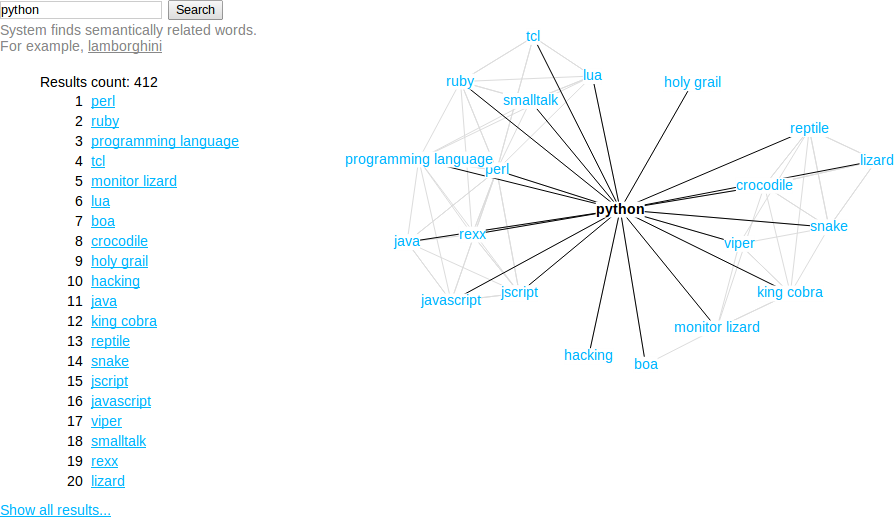
\includegraphics[width=1.0\textwidth]{figures/python}
\end{figure}

\end{frame}




\begin{frame}
\frametitle{Search for Related Words: the List and the Graph}

\begin{figure}
\centering
\includegraphics[height=0.55\textwidth]{../figures/serelex-brussels}
\end{figure}

\end{frame}




\begin{frame}
\frametitle{Search for Related Words: the Images}

\includegraphics[width=1.0\textwidth]{./../figures/citroyen}

\end{frame}

\begin{frame}

\begin{figure}
\frametitle{Evaluation of the Serelex}

\center
\includegraphics[width=0.6\textwidth]{./../figures/satisfaction}

\caption{Users' satisfaction with the top 20 results.}
\end{figure}
\end{frame}


\subsection{Filename Categorization}


\begin{frame}
\frametitle{Related publications}
\begin{itemize}
\item Panchenko A., Naets H., Beaufort R., Fairon C. \textbf{Towards Detection of Child Sexual Abuse Media: Classification of the Associated Filenames}. In Proceedings of the 35th European Conference on Information Retrieval (ECIR 2013).  LNCS 7814, pp. 776-779. Springler-Verlag Berlin Heidelberg 2013.

\item Panchenko A, Beaufort R., Fairon C. \textbf{Detection of Child Sexual Abuse Media on P2P Networks: Normalization and Classification of Associated Filenames}. In Proceedings of Workshop on Language Resources for Public Security Applications of the 8th International Conference on Language Resources and Evaluation (LREC), 2012

\end{itemize}
\end{frame}



\begin{frame}[fragile]
\frametitle{Short text classification with Vocabulary Projection}

\begin{figure}
\center
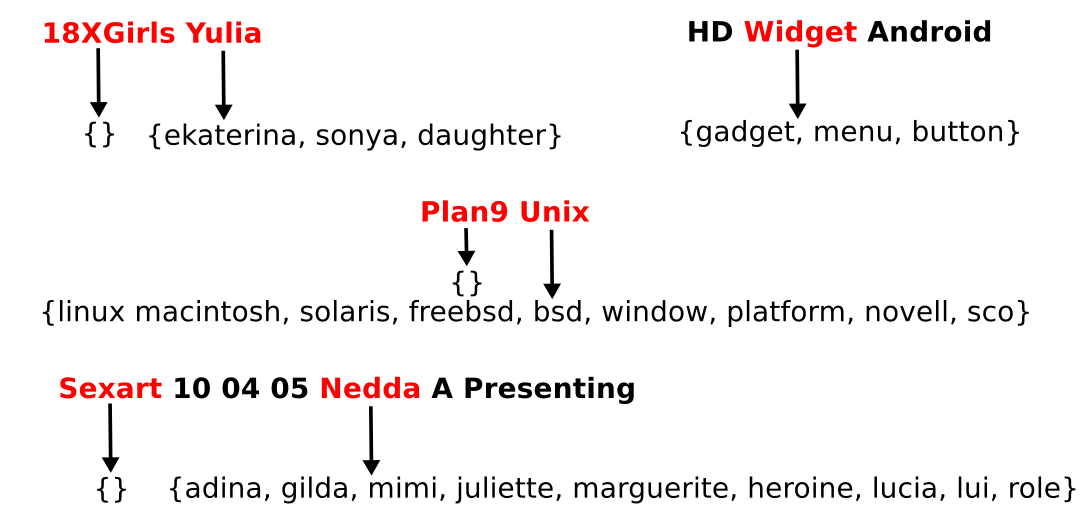
\includegraphics[width=0.9\textwidth]{./figures/vp-ex}
\end{figure}
\end{frame}


\begin{frame}
\frametitle{Evaluation of the Vocabulary Projection}
\begin{table}
\tiny

%\footnotesize
\centering
\begin{tabular}{|l|l|l|l|}

\hline
\bf Training Dataset & \bf Test Dataset & \bf Accuracy  & \textbf{Accuracy (voc. projection)} \\ \hline    

Gallery (train) & Gallery  & 96.41 & \textbf{96.83} (+0.42) \\
PirateBay Title+Desc+Tags & PirateBay Title+Desc+Tags &  \textbf{98.92} &  98.86 (--0.06)\\
PirateBay Title+Tags & PirateBay Title+Tags & \textbf{97.73} & 97.63 (--0.10) \\
Gallery & PirateBay Title+Desc+Tags & 90.57 & \textbf{91.48} (+0.91) \\
\alert{Gallery}  & \alert{PirateBay Title+Tags}  & \alert{84.23} & \alert{\textbf{88.89}} \alert{(+4.66)} \\
PirateBay Title+Desc+Tags & Gallery  & 88.83 & \textbf{89.04} (+0.21) \\
PirateBay Title+Tags & Gallery & 91.16 & \textbf{91.30} (+0.14) \\
\hline

\end{tabular}
\caption{ Performance of an C-SVM linear classifier (10-fold cross validation). }
\label{tbl:results2}

\end{table}
\end{frame}



